\section{Démarche de Modélisation}
\subsection{Le robot poisson}

Le robot (robot poisson ou poisson) simulé est composé de 5 électrodes pour faire de l'\textit{électrolocation active}, c'est-à-dire pour générer un champ électrique qui réagit à l'environnement, tout comme le \textit{Gnathonemus petersii} fait. La suivante figure en deux dimension (le 5-ième capteur n'est pas représenté) montre le robot poisson simulé, ainsi que l'emplacement des électrodes. 

\begin{figure}[h!]
    \centering
    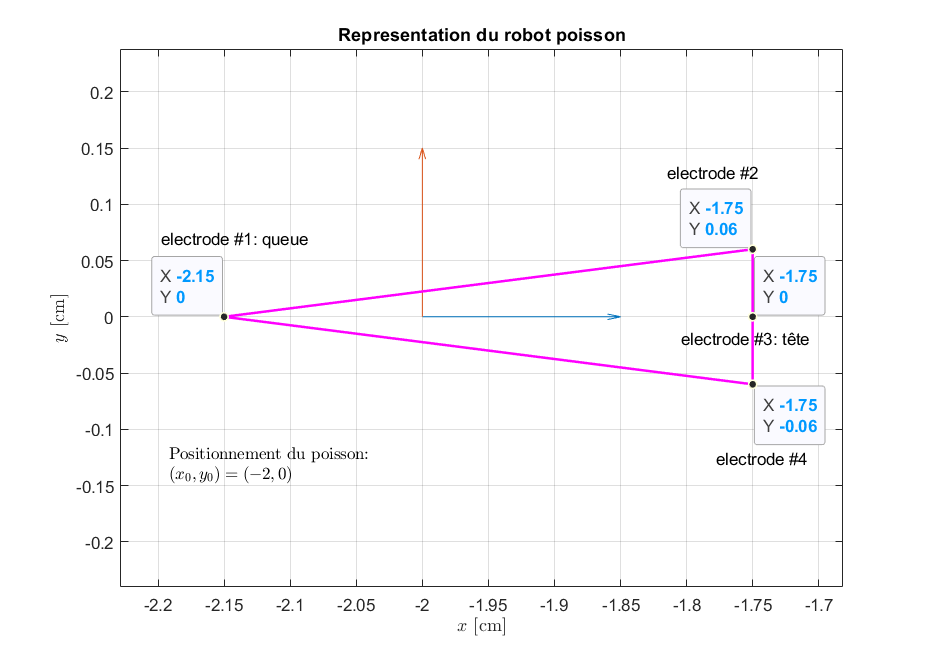
\includegraphics[width=\textwidth]{assets/poisson/poisson.png}
    \caption{Représentation du robot poisson et des capteurs dans le simulateur MATLAB}
    \label{fig:poisson}
\end{figure}

\subsection{La méthode des réflexions}
La méthode des réflexions est une solution au problème d'électrolocation directe, présentée sur \cite{Boyer2012}. Cette technique consiste à résoudre l'équation de Laplace $\Delta\phi = 0$ dans un scénario avec plusieurs objets autour du capteur et avec certaines conditions imposées aux objets (capteur inclus). En appliquant le principe de superposition présenté, dû la rapide atténuation des réflexions $\phi_i$ avec la distance, le vecteur de courants total peut être évalué en considérant jusqu'à la deuxième réflexion: 

\begin{equation}
    \mathbf{I} \approx \mathbf{I}^{(0)} + \mathbf{I}^{(1)} + \mathbf{I}^{(2)}
\end{equation}
où, $\mathbf{I}^{(0)}$ représente les courants mesurés en absence d'objet dans la scène, $\mathbf{I}^{(1)}$ représente les courants réfléchis par l'objet (en absence de capteur dans la scène) et  $\mathbf{I}^{(2)}$ représente la réponse électrique que le capteur génère afin de retrouver son équilibre électrique sous l'excitation de la première réflexion, d'après \cite{Boyer2013}. La Figure \ref{fig:reflexions} résume bien le principe de cette méthode itérative. Chaque potentiel $\phi_i$ représente la réponse à la somme des potentiels $\phi_0 + \phi_1 + \dots \phi_{i-1}$ réfléchis par les objets qui entourent le capteur, et le capteur. Par conséquent, le problème se réduit à trouver les courants associés au potentiel de base $\phi_0$, la première et la seconde réflexion: $\mathbf{I}^{(0)}, \mathbf{I}^{(1)}$ et $\mathbf{I}^{(2)}$. 
\clearpage 
\begin{figure}[h!]
    \centering
    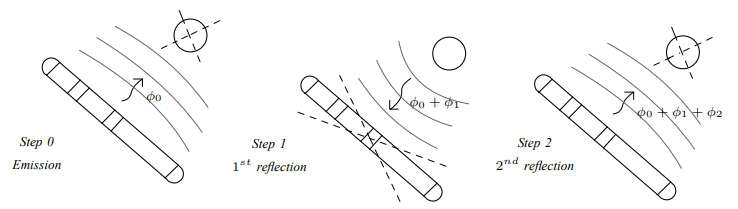
\includegraphics[width=0.8\textwidth]{doc/img/reflexions.png}
    \caption{Schéma des trois premières réflexions de la Méthode des Réflexions, image de \cite{Boyer2012}}
    \label{fig:reflexions}
\end{figure}

D'après \cite{BENACHENHOU}, le courant $\mathbf{I}^{(0)}$ peut être obtenu en utilisant un simulateur numérique et s'écrit: 

\begin{equation}
    \mathbf{I}^{(0)} = \bar{\mathbf{C}}^{(0)} \cdot \mathbf{U}
\end{equation}
avec $\mathbf{U}$ étant le vecteur tension des électrodes, dans notre cas $\mathbf{U} = \left [1, 0, 0, 0, 0 \right ]$ car seulement l'électrode à la queue est alimenté, et $\bar{\mathbf{C}}^{(0)}$ étant la matrice de conductances à vide entre chaque électrode et ayant la suivante forme dans notre cas: 
\begin{center}
$\bar{\mathbf{C}}^{(0)} = \gamma \cdot 
\begin{pmatrix}
0.2557 & -0.0639 & -0.0639 & -0.0639 & -0.063 \\
-0.0639 & 0.1218 & -0.0203 & -0.0173 & -0.0203 \\
-0.0639 & -0.0203 & 0.1218 & -0.0203 & -0.0173 \\
-0.0639 & -0.0173 & -0.0203 & 0.1218 & -0.0203 \\
-0.0639 & -0.0203 & -0.0173 & -0.0203 & 0.1218 \\
\end{pmatrix}$
\end{center}
avec $\gamma$ la conductivité de l'eau $\left ( \text{en } \frac{S}{cm} \right )$.

Les courants $\mathbf{I}^{(1)}$ et $\mathbf{I}^{(2)}$ doivent être calculés en temps réel car ils dépendent de la position du capteur et du reste des objets. Nous divisons le courant généré par les réflexions en une composante axiale et une composante latérale. D'après \cite{Boyer2012}, \say{ la composante axiale $\mathbf{I}_{\text{ax}}$ traduit la réaction du capteur aux différences de potentiel réfléchies par l'objet et évaluées le long de l'axe du capteur, et la composante latérale $\mathbf{I}_{\text{lat}}$ traduit la polarisation latérale du capteur générée par le flux latéral du champ renvoyé par l'objet }: 

\begin{equation}
    \mathbf{I} = \mathbf{I}_{\text{ax}} + \mathbf{I}_{\text{lat}}
\end{equation}
avec
\begin{equation}
    \mathbf{I}_{\text{ax}} = \left ( 1- \bar{\mathbf{C}}^{(0)} \cdot \mathbf{K} \right ) \cdot \mathbf{P}_{+} \cdot \mathbf{I}^{(0)}
\end{equation}
et 
\begin{equation}
    \mathbf{I}_{\text{lat}} = \mathbf{P}_{\perp} \cdot \mathbf{L} \cdot \mathbf{P}_{+} \cdot \mathbf{I}^{(0)}
\end{equation}
où, la matrice $\mathbf{P}_{+}$ projette les courants à travers chaque électrode, en additionnant les courants de la même électrode, la matrice diagonale $\mathbf{P}_{\perp}$ dépend de la géométrie du capteur, et les matrices $\mathbf{K}$ et $\mathbf{L}$ dépendent de la géométrie de l'objet et de sa position et orientation par rapport au capteur. 

Dans le simulateur, nous utilisons la suivante formule pour le calcul des courants mesurées:

\begin{equation}
    \mathbf{I}= \bar{\mathbf{C}}^{(0)} \cdot \mathbf{U} \left ( 1- \bar{\mathbf{C}}^{(0)} \cdot \mathbf{K} \right )
\end{equation}

Ensuite, nous définissons les composantes perturbées des courants $\delta I$ induits par la présence d'un objet proche pour les électrodes à la gauche et la droite de la tête du robot poisson, comme suit: 
\begin{equation}
    \delta I_2 = I_2 - I_{02} \quad ; \quad \delta I_4 = I_4 - I_{04}
\end{equation}
avec $I_2$ et $I_4$ les courants mesurées dans un instant donnée et $I_{02}$ et $I_{04}$ les courants mesurées en absence d'objet proche. 

Et, dans le cas de notre configuration d'électrodes, nous pouvons paramétrer les courants perturbés $\delta I$ par sa composante axiale et sa composante latérale: 

\begin{equation}\label{eq:axial_lateral}
    \delta I_{ax} = \frac{\delta I_1 + \delta I_2}{2} \quad ; \quad \delta I_{lat} = \frac{\delta I_1 - \delta I_2}{2}
\end{equation}

Le scalaire axial $\delta I_{ax}$ nous permet savoir si la scène est composée d'un objet isolant ou conducteur à partir de son signe, tandis que le scalaire latéral $\delta I_{lat}$ nous donne une idée de la position de l'objet par rapport au capteur à partir de son signe. La suivante table regroupe ces idées: 

\begin{table}[h!]
    \centering
    \begin{tabular}{|c|c|c|}
        \hline
        \multirow{2}{*}{$\delta I_{ax}$} & $>0$ & pour un objet conducteur\\ \cline{2-3}
         & $<0$& pour un objet isolant \\
         \hline
         \multirow{4}{*}{$\delta I_{lat}$} & \multirow{2}{*}{$>0$} & pour un objet conducteur à la gauche du capteur \\
          & & \textbf{ou} pour un objet isolant à la droite du capteur \\ \cline{2-3}
          & \multirow{2}{*}{$<0$} & pour un objet conducteur à la droite du capteur \\
          & & \textbf{ou} pour un objet isolant à la gauche du capteur \\
          \hline
    \end{tabular}
    \caption{\centering Propriétés des courants axiaux $\delta I_{ax}$ et latéraux $\delta I_{lat}$ perturbées, de \cite{Boyer2013}}
    \label{tab:proprietes}
\end{table}

Nous utiliserons cette table pour vérifier notre simulateur plus tard, dans la Section \ref{sec:resultats}, et pour définir une loi de contrôle, dans la Section \ref{sec:controle}.

Dans ce qui suit, nous devons calculer la matrice $\mathbf{K}$ pour les différents objets que le capteur peut rencontrer. Nous allons considérer uniquement le cas d'un petit objet qui peut être isolant ou conducteur, et le cas d'un mur isolant. Notre simulateur placera des objets dans l'aquarium composé de 4 murs isolants. 

\subsubsection{Cas d'un petit objet}
Pour le calcul de la matrice $\mathbf{K}$ dans le cas d'un petit objet, nous prenons en compte le scénario composé d'un capteur (ou une électrode $\varepsilon_{\alpha}$), qui a pour centre $x_\alpha$, et d'un petit objet $\mathbf{p}$, qui lui a pour centre $y_c$.
\begin{figure}[h!]
    \centering
    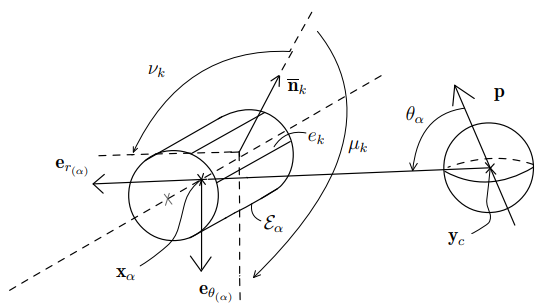
\includegraphics{doc/img/schema_petit_objet.png}
    \caption{\centering Schéma représentant la macro-électrode $\varepsilon_{\alpha}$ du capteur perturbée par une sphère $\mathbf{p}$.}
    \label{fig:schema_petit_objet}
\end{figure}
Il est prouvé dans \cite{Boyer2012} que la matrice $\mathbf{K}$ de réponse à cet objet suit l'expression suivante: 
\begin{equation}
    \mathbf{K}_{\text{objet}} = - \frac{1}{4\pi \cdot \gamma} \cdot \frac{\mathbf{r}_\alpha \cdot \mathbf{P}_r \cdot \mathbf{r}_\beta}{\lVert \mathbf{r}_\alpha \rVert^3 \cdot \lVert \mathbf{r}_\beta \rVert^3}
\end{equation}
où, $\mathbf{r}_\alpha = y_c - x_\alpha$, c'est-à-dire la distance entre l'objet et le capteur considéré, $\mathbf{r}_\beta = y_c - x_\beta$, c'est-à-dire la distance entre l'objet et un autre capteur, et $\mathbf{P}$ le tenseur de polarisation qui dépend de la géométrie de l'objet et du caractère conducteur/isolant. Pour une sphère, $\mathbf{P} = \upchi \cdot a^3 \cdot \mathbf{I}_{3}$ avec $\mathbf{I}_3$ la matrice identité de $3$ dimensions, $a$ le rayon de la sphère et $\upchi$ le facteur de contraste: $1$ pour un objet totalement conducteur et $-0.5$ pour un objet totalement isolant.

Lors de la révision des résultats, vous trouverez la forme des courants lorsque le robot poisson s'approche à un objet totalement isolant et un objet totalement conducteur. 

\subsubsection{Cas d'un mur isolant}

Pour le cas des murs, nous utilisons la méthode présenté dans \cite{Jackson2012} pour des objets de grande taille. Comme illustré dans la Figure \ref{fig:schema_murs_coins}, cette méthode consiste à créer une image virtuelle du robot placée symétriquement au mur, qui a pour centre $x_\beta^*$ et, dans le cas d'approximation à un coin, une troisième image placée symétriquement au coin $C$. 

\begin{figure}[h!]
    \centering
    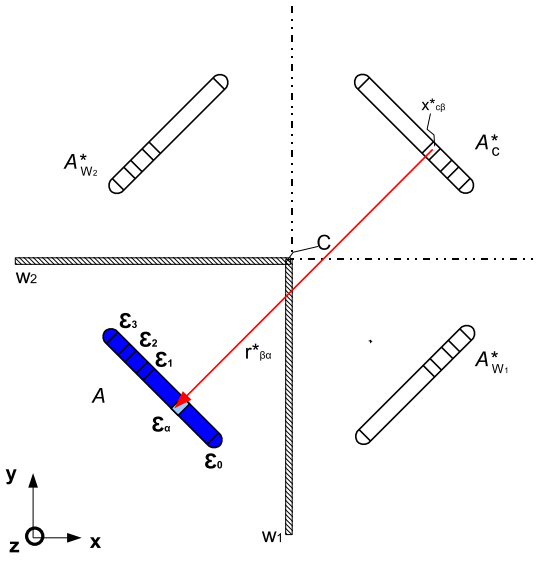
\includegraphics[scale=0.5]{doc/img/schema_murs_coins.png}
    \caption{\centering Schéma représentant le capteur $A$ et les images virtuelles $A_{W_1}^*$ et $A_{W_2}^*$ symétriques aux murs $W_{1}$ et $W_{2}$, respectivement, et l'image virtuelle $A_C^*$ symétrique par rapport au coin $C$. }
    \label{fig:schema_murs_coins}
\end{figure}

En considérant le potentiel généré par le mur comme la superposition du champ du robot et le champ de son image, nous obtenons la matrice $\mathbf{K}$ de réponse aux murs suivante: 

\begin{equation}
    \mathbf{K}_{\text{murs}} = - \frac{1}{4\pi \cdot \gamma} \cdot \frac{1}{\lVert \mathbf{r}_{\beta\alpha}^* \rVert^3}
\end{equation}
où, $\mathbf{r}_{\beta\alpha}^* = x_\alpha - x_\beta^*$ pour chaque combinaison d'électrode réel et électrode image. Du fait que notre aquarium porte 4 murs, nous avons 8 réflexions au total (4 réflexions provenant des murs et 4 réflexions provenant des coins). Dans la Figure \ref{fig:wall_reflexion} nous pouvons voir une représentation des 8 images virtuelles du robot poisson par rapport aux murs et aux coins. 

\begin{figure}
    \centering
    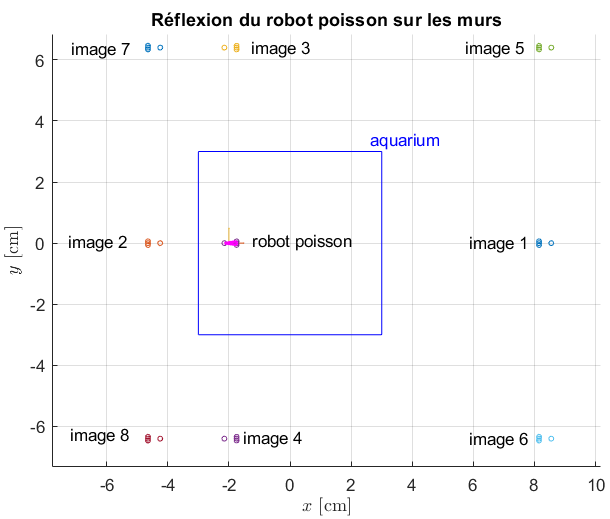
\includegraphics[scale=0.8]{assets/wall_reflexions/wall_reflexion.png}
    \caption{\centering Réflexions du robot poisson par rapport aux murs et aux coins.}
    \label{fig:wall_reflexion}
\end{figure}
\clearpage

\subsection{Résultats obtenus} \label{sec:resultats}
Cette section montre les résultats obtenus lors de certaines simulations, et comme avancé précédemment, nous permettent de vérifier le calcul des courants avec la Table \ref{tab:proprietes}. 

L'allure de certaines courbes peuvent être endommagés par la présence de l'objet (isolant ou conducteur) à la position $(x,y) = (2.5, 2.5)$, mais le simulateur créée a besoin d'un objet isolant et d'un objet conducteur pour que les matrices $\mathbf{K}$ calculées soient pas égales à $0$.

\subsubsection{Cas d'un petit objet conducteur}
\begin{figure}[h!]
    \centering
    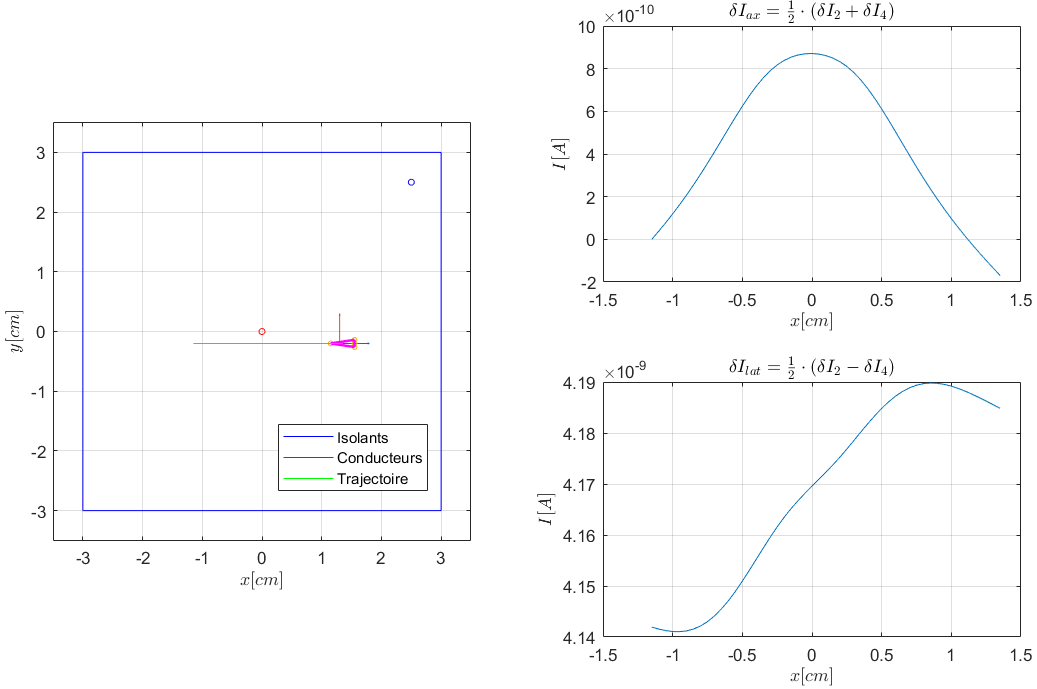
\includegraphics[width=\textwidth]{assets/plot_currents/Table1/conducteur_bas.png}
    \caption{\centering Représentation de la trajectoire suivi par le robot poisson (à gauche) et graphiques du courant axial $\delta I_{ax}$ et latéral $\delta I_{lat}$ en fonction de la distance parcourue dans l'axe $X$ (à droite).}
    \label{fig:conducteur_bas}
\end{figure}

\begin{figure}[h!]
    \centering
    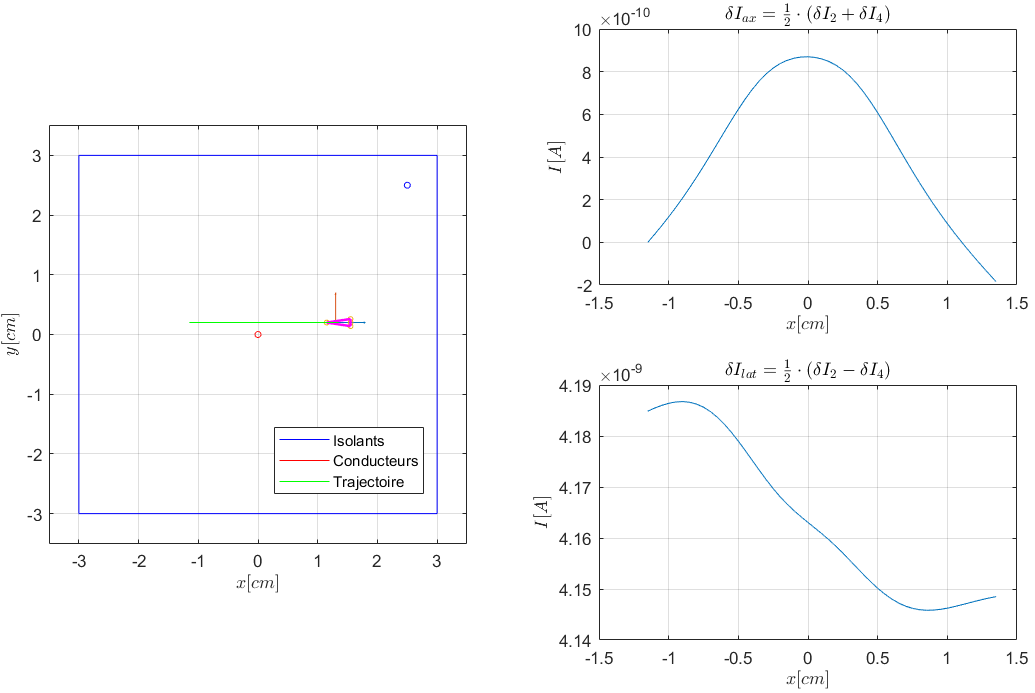
\includegraphics[width=\textwidth]{assets/plot_currents/Table1/conducteur_haut.png}
    \caption{\centering Représentation de la trajectoire suivi par le robot poisson (à gauche) et graphiques du courant axial $\delta I_{ax}$ et latéral $\delta I_{lat}$ en fonction de la distance parcourue dans l'axe $X$ (à droite).}
    \label{fig:conducteur_haut}
\end{figure}
\clearpage
\subsubsection{Cas d'un petit objet isolant}
\begin{figure}[h!]
    \centering
    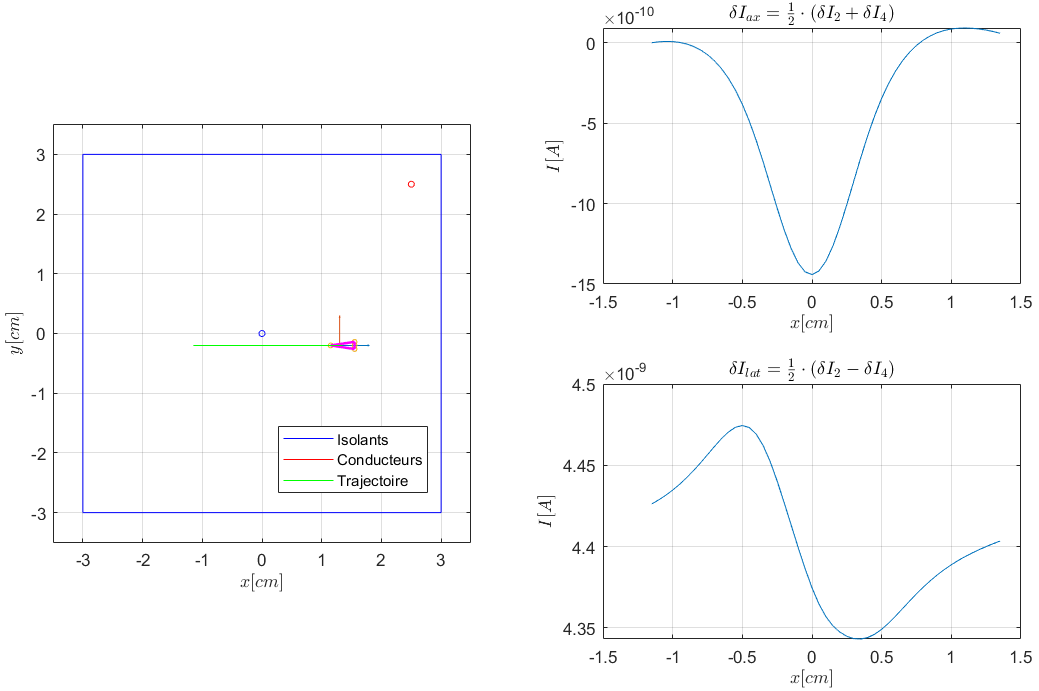
\includegraphics[width=\textwidth]{assets/plot_currents/Table1/isolant_bas.png}
    \caption{\centering Représentation de la trajectoire suivi par le robot poisson (à gauche) et graphiques du courant axial $\delta I_{ax}$ et latéral $\delta I_{lat}$ en fonction de la distance parcourue dans l'axe $X$ (à droite).}
    \label{fig:isolant_bas}
\end{figure}
\begin{figure}[h!]
    \centering
    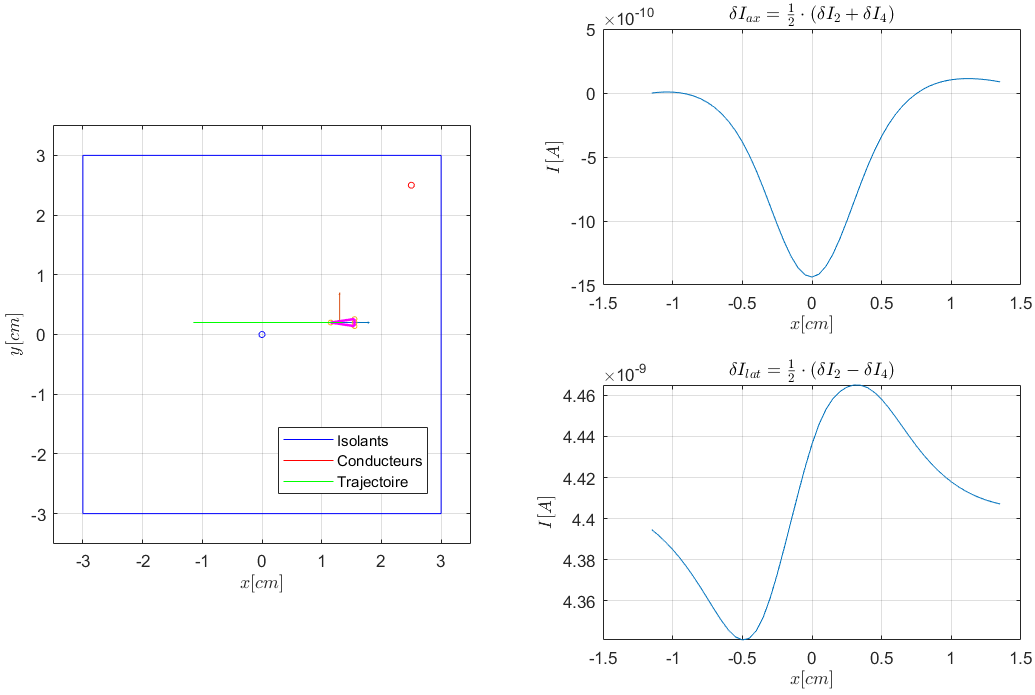
\includegraphics[width=\textwidth]{assets/plot_currents/Table1/isolant_haut.png}
    \caption{\centering Représentation de la trajectoire suivi par le robot poisson (à gauche) et graphiques du courant axial $\delta I_{ax}$ et latéral $\delta I_{lat}$ en fonction de la distance parcourue dans l'axe $X$ (à droite).}
    \label{fig:isolant_haut}
\end{figure}

%\clearpage
%\subsubsection{Cas d'un mur (isolant)}
%\begin{figure}[h!]
%    \centering
%    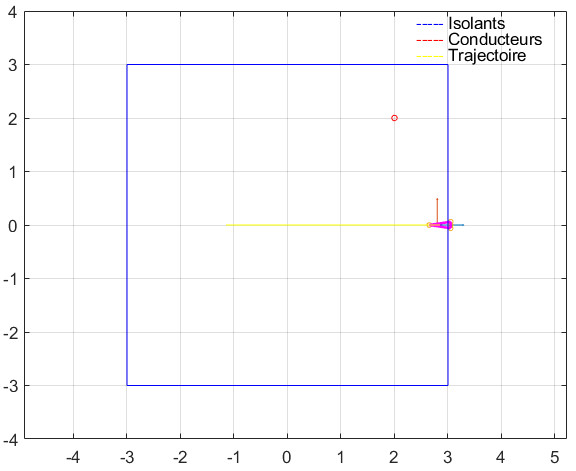
\includegraphics[width=0.5\textwidth]{assets/plot_currents/approximation_wall/approximation_wall_trajectoire.png}
%    \caption{Représentation de l'aquarium pour la simulation. En bleu, les objets isolants (murs et objet), en rouge les objets conducteurs et en jaune la trajectoire suivi par le robot poisson.}
%    \label{fig:approximation_wall_trajectoire}
%\end{figure}
%\begin{figure}[h!]
%    \centering
%    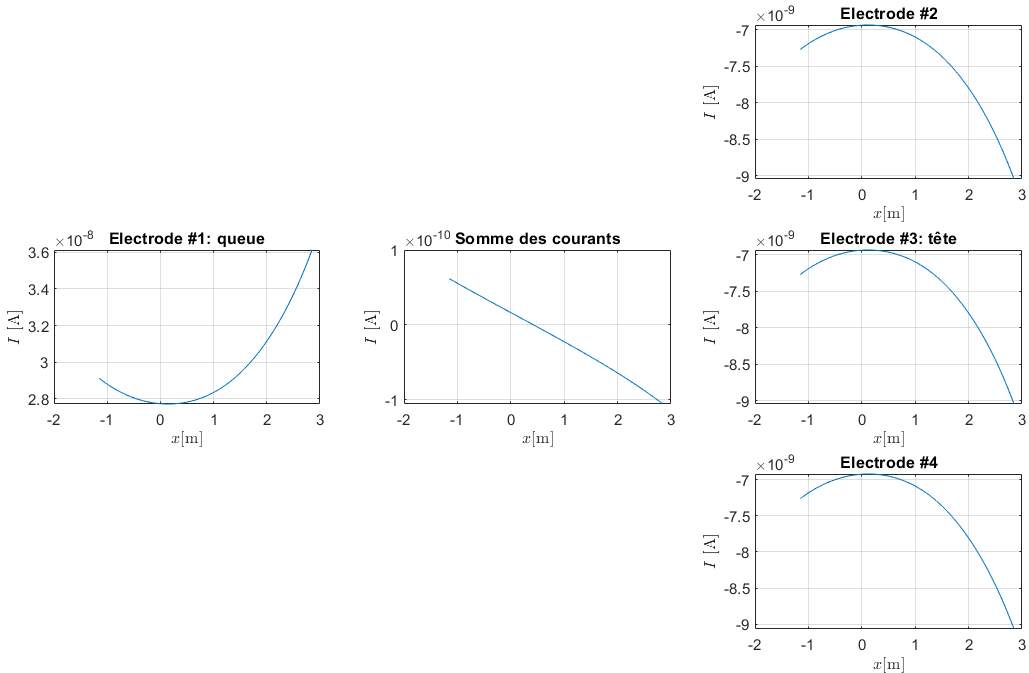
\includegraphics[width=0.9\textwidth]{assets/plot_currents/approximation_wall/approximation_wall.png}
%    \caption{Courants obtenus dans l'électrode \#1 (queue), \#2, \#3 (tête) et \#4, lors de l'approximation à un mur.}
%    \label{fig:approximation_wall}
%\end{figure}